\documentclass[11pt]{article}
\usepackage[margin=1in]{geometry}
\usepackage{amsmath,amssymb}
\usepackage{booktabs}
\IfFileExists{siunitx.sty}{\usepackage{siunitx}}{\def\NoSiunitx{1}}
\ifdefined\NoSiunitx
  \newcommand{\volt}{\mathrm{V}}\newcommand{\ampere}{\mathrm{A}}
  \newcommand{\ohm}{\Omega}
  \newcommand{\kilo}{\mathrm{k}}\newcommand{\milli}{\mathrm{m}}
  \newcommand{\micro}{\mu}\newcommand{\nano}{\mathrm{n}}
  \newcommand{\per}{/}
  \newcommand{\SI}[2]{\ensuremath{#1\,#2}}
  \newcommand{\SIrange}[3]{\ensuremath{#1\text{--}#2\,#3}}
\fi
\usepackage{enumitem}
\usepackage{graphicx}
\usepackage{xcolor}
\usepackage[colorlinks=true,linkcolor=blue,urlcolor=blue]{hyperref}

\newcommand{\Ven}{V_{\mathrm{EN}}}
\newcommand{\Vref}{V_{\mathrm{REF}}}
\newcommand{\Vtlv}{V_{\mathrm{TLV}}}
\newcommand{\Vth}{V_{\mathrm{EN,th}}}
\newcommand{\Iref}{I_{\mathrm{ref}}}
\newcommand{\Istby}{I_{\mathrm{STBY}}}
\newcommand{\Ihys}{I_{\mathrm{HYS}}}
\newcommand{\IH}{I_{H}}
\newcommand{\Rone}{R_{1a}}
\newcommand{\Rtwo}{R_{1b}}
\newcommand{\Rt}{R_{2}}
\newcommand{\Von}{V_{\mathrm{on}}}
\newcommand{\Voff}{V_{\mathrm{off}}}
\newcommand{\Vlatch}{V_{\mathrm{latch}}}

\title{LM5176 \texttt{EN/UVLO} Threshold with TLV431 Latch:\\
Equations, Ranges, and Design Constraints}
\author{USB-C PD $\to$ 12\,V Fan-Array Controller --- Buck-Boost 42\,W}
\date{}

\begin{document}
\maketitle

\begin{abstract}
\noindent
This document derives the equations and worst-case design constraints for the
three-resistor \texttt{EN/UVLO} divider that feeds both the LM5176 enable pin
and the TLV431 reference of the external lockout latch. It is the analytical
companion to \texttt{10a\_uvlo\_resistor\_search.py}, which searches stocked
resistor values against these constraints. The latch circuit itself is
documented in \texttt{uvlo\_latch.tex} / \texttt{10b\_uvlo\_latch.py}.

\smallskip\noindent
\textbf{Result:} $\Rt/\Rone/\Rtwo = 420/150/15\,\mathrm{k}\Omega$
($\Rt$ = 120\,k $+$ 300\,k in series), guaranteed turn-on band
2.75--\SI{4.49}{\volt}, per-unit gaps $52/\SI{41}{\milli\volt}$.
\end{abstract}

\section{Motivation: why an external lockout latch}

The LM5176 advertises pre-biased startup, but in this design it does not
survive an input dropout in practice. The control loop is deliberately slow
(low crossover frequency, chosen so the loop does not react to the fan
commutation pulses --- see the stability notebook), and with that loop the part
misbehaves when $V_{IN}$ recovers while the output capacitors are still charged:
the restart into a pre-biased output is not handled cleanly. TI support was
unable to root-cause the failure; their only suggestion was to raise the
crossover frequency, which is ruled out by the system requirement that set the
low crossover in the first place --- the loop must not chase the fan
commutation pulses, so raising its bandwidth would trade one problem for
another.

The chosen fix is a small discrete latch: on an input dropout it pulls
\texttt{EN/UVLO} low and, because it is \emph{powered from} $V_{OUT}$, it
holds \texttt{EN/UVLO} low until the output has actually discharged. Every
restart therefore begins from a nearly dead output and the pre-bias path is
never exercised. This document sizes the divider that tells the latch
\emph{when} to fire; the latch itself is in \texttt{uvlo\_latch.tex}.

\section{Circuit topology and conventions}

A single node, \texttt{EN/UVLO} (voltage $\Ven$), is driven from $V_{IN}$ through
$\Rt$. A two--element lower leg returns to ground: $\Rtwo$ connects \texttt{EN/UVLO}
to the TLV431 reference node (voltage $\Vref$), and $\Rone$ connects that reference
node to ground. The TLV431 \texttt{REF} pin sits on the $\Vref$ node and draws a bias
current $\Iref$ \emph{into} the pin.

\begin{center}
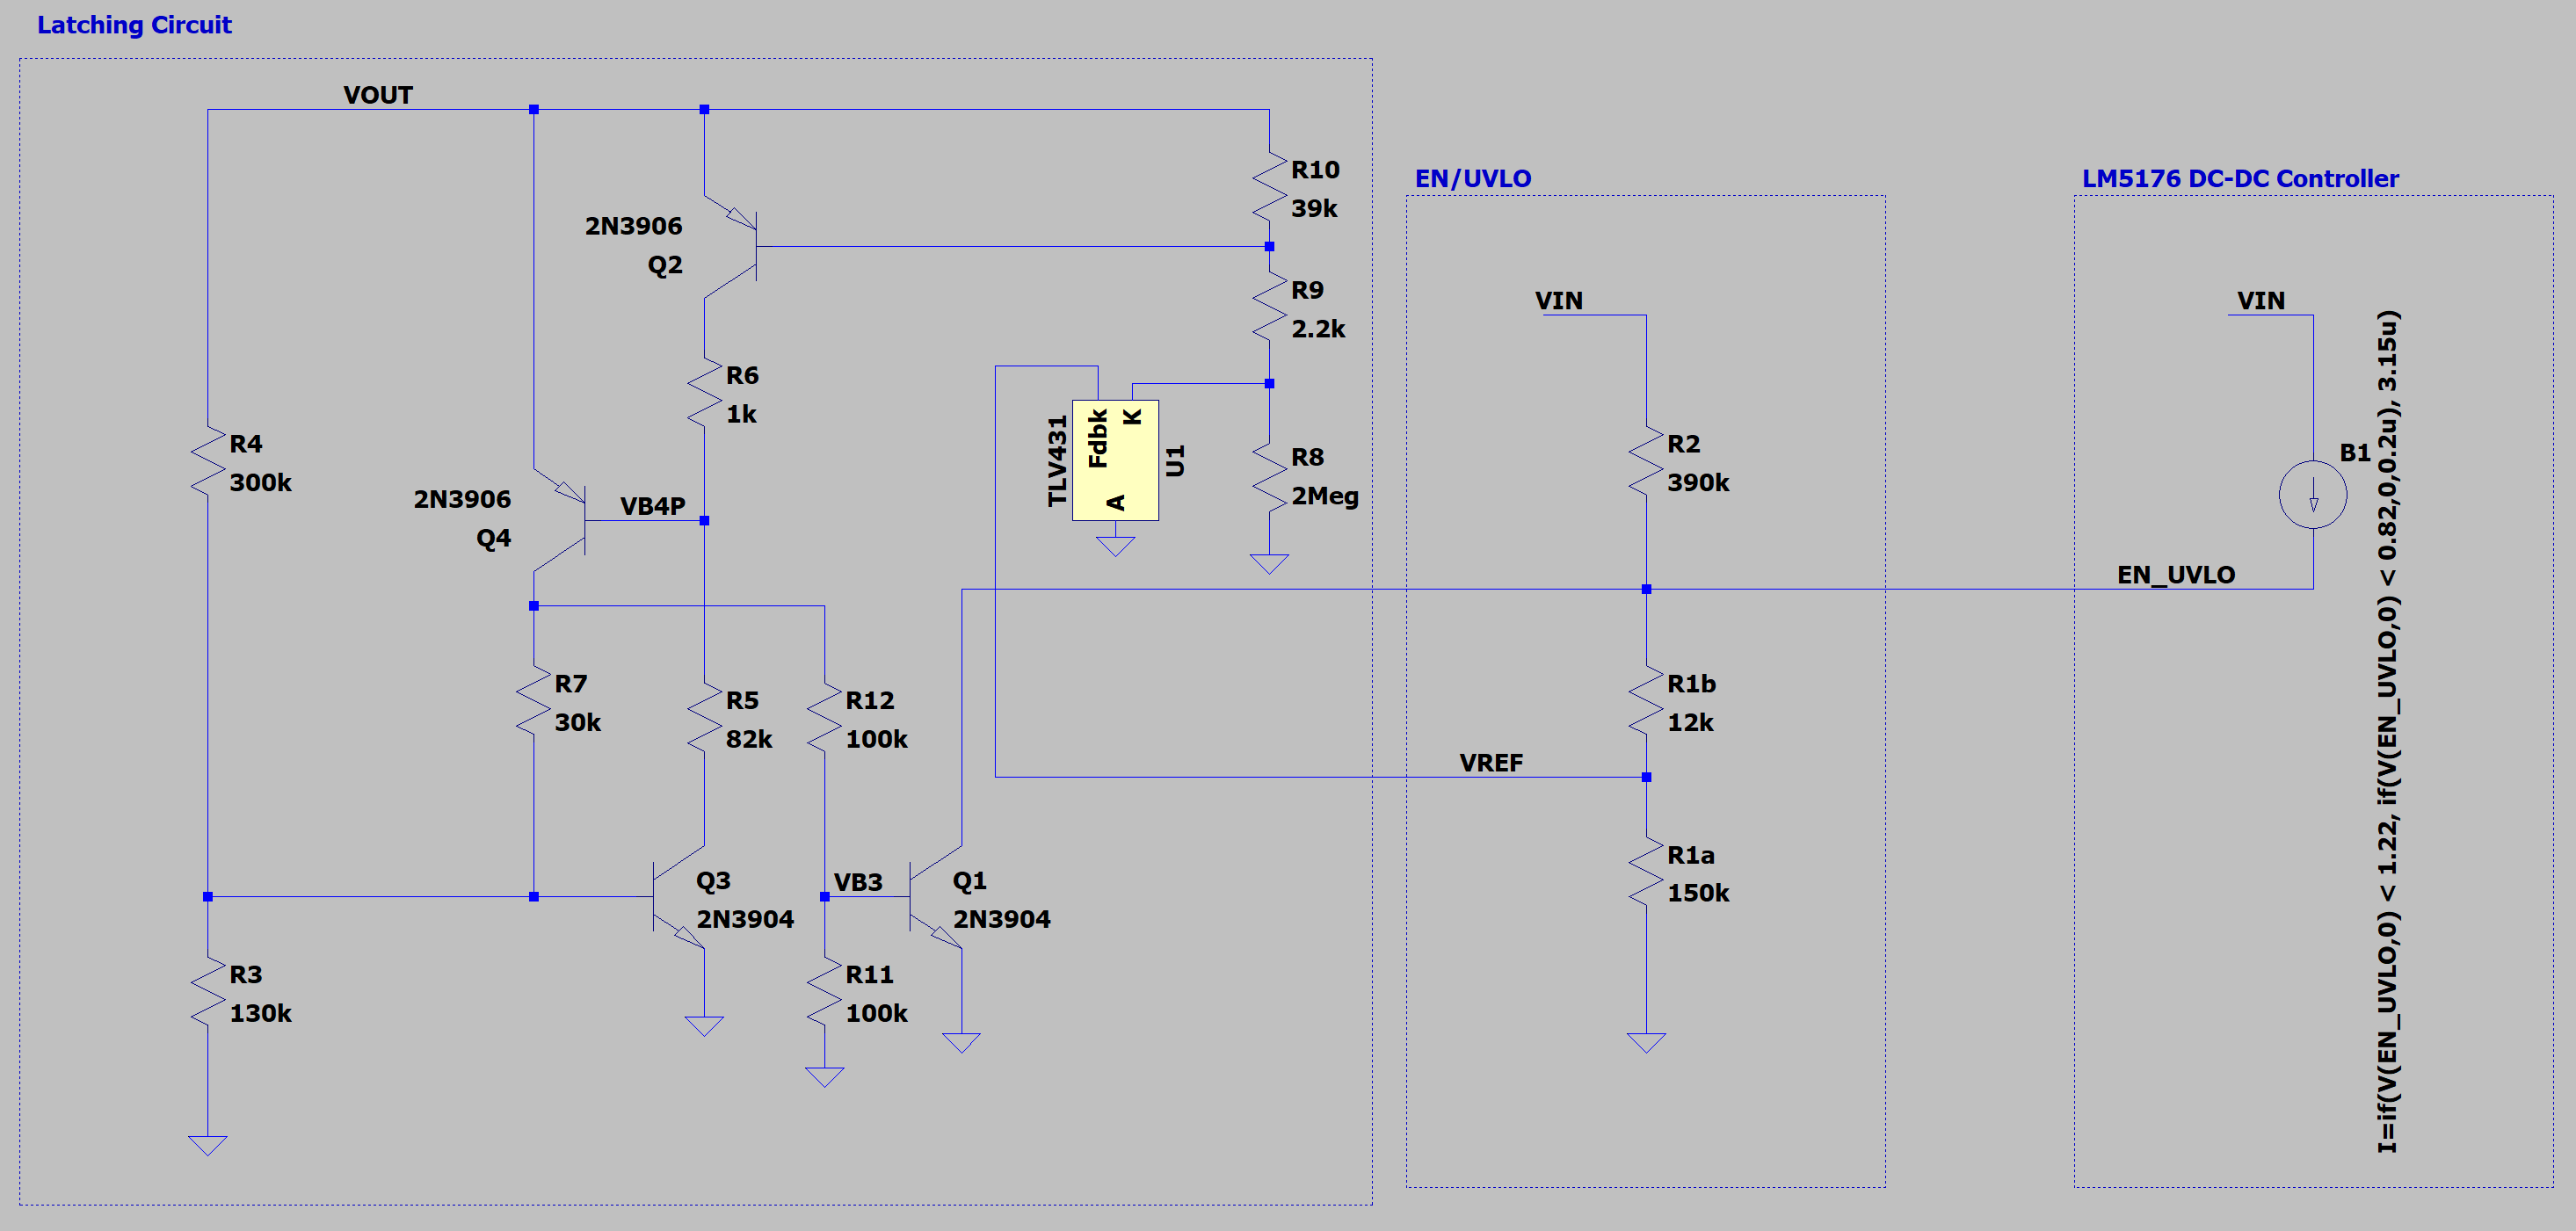
\includegraphics[width=\textwidth]{figures/divider_latch_schematic.png}
\end{center}
\noindent (Left block: the lockout latch of \texttt{uvlo\_latch.tex}; right:
the $\Rt$/$\Rtwo$/$\Rone$ divider on the \texttt{EN/UVLO} pin with the
behavioural EN-current source used in simulation.)

\paragraph{Current--source convention (LM5176).}
Per the datasheet, the LM5176 \emph{sources} current \emph{out of} the
\texttt{EN/UVLO} pin into the node: $\Istby$ in standby, plus an additional
$\Ihys$ once the operating (UVLO) threshold is crossed, which lifts $\Ven$ and
creates the turn-on/turn-off hysteresis. The total injected current is
\[
I_S \;=\; \Istby + \IH,\qquad
\IH=\begin{cases}0 & \text{standby (rising, before turn-on)}\\[2pt]\Ihys & \text{running (after turn-on)}\end{cases}
\]

\section{Parameter ranges}

\begin{center}
\begin{tabular}{lccl}
\toprule
Symbol & Min & Max & Notes \\
\midrule
$V_{IN}$            & \SI{4.5}{\volt}  & \SI{22}{\volt}   & USB input \\
$\Vth$ (operating)  & \SI{1.17}{\volt} & \SI{1.29}{\volt} & LM5176 \texttt{EN/UVLO} operating threshold \\
$\Istby$            & \SI{1}{\micro\ampere}    & \SI{3}{\micro\ampere}    & standby source current \\
$\Ihys$             & \SI{2.15}{\micro\ampere} & \SI{4.25}{\micro\ampere} & added after turn-on \\
$\Iref$             & \SI{0}{\micro\ampere}    & \SI{0.38}{\micro\ampere} & TLV431 \texttt{REF} input current \\
$\Vtlv$             & \SI{1.193}{\volt}& \SI{1.266}{\volt}& effective TLV431 reference (see below) \\
Resistors           & \multicolumn{2}{c}{$\pm3\%$} & budget-derived; see below \\
\bottomrule
\end{tabular}
\end{center}

\paragraph{Effective TLV431 reference $\Vtlv$.}\label{sec:vtlv}
Built up from the nominal \SI{1.24}{\volt}:
\[
\Vtlv^{\max}=1.240+\underbrace{0.0062}_{+0.5\%}+\underbrace{0.020}_{\text{temp}}=\SI{1.266}{\volt},
\qquad
\Vtlv^{\min}=1.240-\underbrace{0.0062}_{-0.5\%}-\underbrace{0.020}_{\text{temp}}-\underbrace{0.021}_{V_{KA}\text{ effect}}=\SI{1.193}{\volt}.
\]
The $V_{KA}$ term uses the datasheet reference shift
$\approx-1.5\,\mathrm{mV/V}$ across the cathode excursion. The
cathode floats to $\approx\SI{15.4}{\volt}$ once the latch fires (see
\texttt{uvlo\_latch.tex}), so the shift spans $1.24\to\SI{15.4}{\volt}$:
$1.5\,\mathrm{mV/V}\times14.2\,\mathrm{V}\approx\SI{21}{\milli\volt}$. The
term only shifts the reference \emph{down}, so it appears in the min only.

\noindent This excursion also drove the choice of vendor: the reference sees
the full $\approx\SI{15.4}{\volt}$ on its cathode whenever the latch is
engaged, so a part rated to only \SI{6}{\volt} on $V_{KA}$ (the TI TLV431)
would be outside its absolute maximum in normal operation of this circuit.
The onsemi TLV431, rated \SI{16}{\volt}, is the part assumed throughout ---
the two are otherwise pin- and function-compatible, which makes this an easy
substitution to get wrong.

\paragraph{Resistor tolerance budget.} $\pm3\%$ everywhere: 1\% purchase
tolerance $+$ $\sim$0.4\% tempco (100\,ppm$/^{\circ}$C over the
0--50$^{\circ}$C range) $+$ $\sim$1.5\% load-life and soldering drift.

\section{Node equations (KCL)}

\paragraph{\texttt{EN/UVLO} node.}
\begin{equation}
\frac{V_{IN}-\Ven}{\Rt}+I_S \;=\; \frac{\Ven-\Vref}{\Rtwo}
\label{eq:kcl_en}
\end{equation}

\paragraph{\texttt{REF} node.}
\begin{equation}
\frac{\Ven-\Vref}{\Rtwo} \;=\; \frac{\Vref}{\Rone}+\Iref
\label{eq:kcl_ref}
\end{equation}

\section{Closed-form solutions}

Solving \eqref{eq:kcl_en}--\eqref{eq:kcl_ref}:

\begin{equation}
\boxed{\;\Ven \;=\; \frac{V_{IN}(\Rone+\Rtwo)+I_S\,\Rt(\Rone+\Rtwo)-\Iref\,\Rone\,\Rt}{\Rone+\Rtwo+\Rt}\;}
\label{eq:ven}
\end{equation}

\begin{equation}
\boxed{\;\Vref \;=\; \frac{\Rone\,(\Ven-\Iref\,\Rtwo)}{\Rone+\Rtwo}\;}
\label{eq:vref}
\end{equation}

\paragraph{TLV431 trip relation (the key design lever).}
The map between $\Ven$ and $\Vref$ depends only on the lower leg, \emph{independent of
$V_{IN}$, $\Rt$, and the EN-pin currents}:
\begin{equation}
\Ven \;=\; \Vref\,\frac{\Rone+\Rtwo}{\Rone}+\Iref\,\Rtwo
\quad\Longrightarrow\quad
\boxed{\;\Ven\big|_{\mathrm{trip}} \;=\; \Vtlv\,\frac{\Rone+\Rtwo}{\Rone}+\Iref\,\Rtwo\;}
\label{eq:ven_trip}
\end{equation}
at the instant $\Vref=\Vtlv$.

\paragraph{Inverting \eqref{eq:ven} for $V_{IN}$.} For any target $\Ven$ in a given state,
\begin{equation}
V_{IN}\;=\;\frac{\Ven(\Rone+\Rtwo+\Rt)-I_S\,\Rt(\Rone+\Rtwo)+\Iref\,\Rone\,\Rt}{\Rone+\Rtwo}.
\label{eq:vin}
\end{equation}

\section{Latch behavior and the three threshold events}\label{sec:events}

The external latch is powered from $V_{OUT}$ and defaults to engaged: it is
held off (\emph{dearmed}) only while $\Vref>\Vtlv$. There is no
``arm-after-first-release'' grace --- whenever $\Vref$ sits below $\Vtlv$ with
the converter running \emph{and $V_{OUT}$ above the latch's arm threshold
($\approx\SI{2.8}{\volt}$ nominal; see \texttt{uvlo\_latch.tex})}, the latch
grabs and pulls \texttt{EN/UVLO} low, holding until $V_{OUT}$ has decayed
($\approx$1--\SI{1.8}{\volt} release). The divider must therefore keep the
TLV431 conducting throughout normal operation.

\begin{enumerate}[nosep]
\item $V_{IN}$ rises; $\Ven$ (standby, $I_S=\Istby$) reaches $\Vth$: LM5176 turns on.
\item $\Ihys$ switches in $\Rightarrow$ $\Ven$, hence $\Vref$, jumps up. Because the
design forces $\Vlatch<\Von$ (constraint~C2), $\Vref$ is already above $\Vtlv$ at
this instant: the latch is dearmed \emph{at} turn-on, even on an arbitrarily slow rise.
\item $V_{IN}$ falls. While running, $\Vref$ falls; when it drops below $\Vtlv$
the latch engages before the LM5176 would reach $\Vth$ on its own (constraint~C3).
\end{enumerate}

\paragraph{Event definitions.} All three events are \textbf{values of $V_{IN}$},
each defined by \eqref{eq:vin} with the $\Ven$ level and EN-pin current of its
own operating state:

\begin{center}
\begin{tabular}{llll}
\toprule
Event & $V_{IN}$ at which\ldots & $I_S$ & state \\
\midrule
$\Von$    & $\Ven=\Vth$ & $\Istby$ & standby, rising (turn-on) \\
$\Vlatch$ & $\Ven=\Ven|_{\mathrm{trip}}$ & $\Istby+\Ihys$ & running, falling (TLV431 trip) \\
$\Voff$   & $\Ven=\Vth$ & $\Istby+\Ihys$ & running, falling (LM5176 self-dropout) \\
\bottomrule
\end{tabular}
\end{center}

The required ordering, for every individual unit, is
\begin{equation}
\Voff\;<\;\Vlatch\;<\;\Von .
\label{eq:order}
\end{equation}
Note the chain deliberately mixes states: $\Von$ uses the \emph{standby}
current because that is the state the part is actually in as $V_{IN}$ rises;
the moment the threshold is crossed, $\Ihys$ engages and $\Ven$ jumps
\emph{upward} (the equivalent running-state crossing is $\Voff$, lower by the
hysteresis), so comparing $\Vlatch$ (a running event) against the standby
$\Von$ is the correct and conservative form for the turn-on race.

\paragraph{Equivalent chain in $\Vref$.} Because running-state $\Vref$ is
monotonic in $V_{IN}$, \eqref{eq:order} is equivalent to bracketing the TLV431
reference between the running-state $\Vref$ levels at the two LM5176 events:
\begin{equation}
\underbrace{\frac{\Rone(\Vth-\Iref\Rtwo)}{\Rone+\Rtwo}}_{\Vref^{\mathrm{run}}\ \text{at}\ \Voff}
\;<\;\Vtlv\;<\;\Vref^{\mathrm{run}}\ \text{at}\ \Von ,
\label{eq:order_ref}
\end{equation}
i.e.\ the TLV431 must still be conducting when the LM5176 would drop out
(left), and must be conducting from the moment $\Ihys$ engages at turn-on
(right) --- the requirement begins once $\Ihys$ lifts the running-state
$\Vref$, which happens as (or just before) the converter starts switching.

\section{Design constraints (worst case)}

Each must hold across the $\pm3\%$ resistor tolerance and every chip-parameter
extreme of the table above.

\paragraph{C1 --- Guaranteed turn-on by \SI{4.5}{\volt}.}
In standby,
\begin{equation}
\min \;\Ven\big(V_{IN}{=}4.5,\;I_S{=}\Istby^{\min},\;\Iref^{\max}\big)\;\ge\;\Vth^{\max}=\SI{1.29}{\volt}.
\end{equation}

\paragraph{C2 --- Latch dearmed below turn-on (per-unit).}
\begin{equation}
\min_{\text{corners}}\big(\Von-\Vlatch\big)\;\ge\;0 .
\label{eq:c2}
\end{equation}
We require $\Von>\Vlatch$ so that no band exists in which the converter runs
while $\Vref<\Vtlv$ (such a band would let the default-engaged latch grab
during a slow start). Like C3, \eqref{eq:c2} is a per-unit
(correlated) difference --- evaluated as one subtraction per device, never as a
gap between independent population bands (Section~\ref{sec:corr}).

\paragraph{C3 --- Latch fires before the LM5176's own UVLO (per-unit).}
\begin{equation}
\min_{\text{corners}}\big(\Vlatch-\Voff\big)\;\ge\;0 .
\label{eq:c3}
\end{equation}

\paragraph{C4 --- Do not turn on too early.}
The worst-case \emph{earliest} turn-on must stay above
$V_{\mathrm{on}}^{\min}\ge\SI{2.5}{\volt}$, so a not-yet-settled USB rail is not
loaded and the converter is not asked to boost from an impractically low input.
C4 fights C2: the large $\Rt$ that C2 demands, together with the
\SIrange{1}{3}{\micro\ampere} spread of $\Istby$, smears turn-on across a
$\sim$\SI{1.5}{\volt} band and drags the earliest turn-on down.

\paragraph{The hysteresis budget links C2 and C3.}
From \eqref{eq:vin}, $\partial V_{IN}/\partial I_S=-\Rt$ exactly, so the two
$\Ven=\Vth$ crossings, whose currents differ by $\Ihys$, are separated by
\begin{equation}
\Von-\Voff=\Ihys\,\Rt .
\label{eq:hyst}
\end{equation}
Subtracting $(\Vlatch-\Voff)$ from both sides,
\begin{equation}
\boxed{\;\big(\Von-\Vlatch\big)\;=\;\Ihys\Rt\;-\;\big(\Vlatch-\Voff\big)\;}
\label{eq:budget}
\end{equation}
--- the two gaps share the single budget $\Ihys\Rt$. A larger $\Rt$ widens the
budget, \emph{and} the $\Vth$ ($\pm\SI{60}{\milli\volt}$) and $\Vtlv$
($+26/-\SI{47}{\milli\volt}$ about \SI{1.24}{\volt}) spreads inflate the worst-case
$(\Vlatch-\Voff)$ gap by the factor $(\Rone+\Rtwo+\Rt)/(\Rone+\Rtwo)$
(Section~\ref{sec:corr}, Eq.~\eqref{eq:gap}). Fitting that inflated gap inside
the budget while leaving $(\Von-\Vlatch)\ge0$ is what forces $\Rt$ large ---
and a large $\Rt$ means a low, soft turn-on with divider current sinking toward
the EN bias currents. The search rejects the \emph{bias-dominated} region
(divider current at turn-on below the total EN bias current) because there
$\Ven$ becomes dominated by $\Istby/\Ihys$ --- currents with wide spec spreads
and no drift specification --- so the thresholds would smear with current
spread rather than track $V_{IN}$. The net effect is that all four constraints
together are satisfiable only in a narrow design band --- a real consequence of
the part tolerances, not a modelling artifact.

\paragraph{Worked result ($\pm3\%$, corrected $\Vtlv^{\min}$).}
Restricting the search to JLCPCB basic-part 0603 values, \emph{no} triple of
single stocked resistors clears all four constraints. Allowing $\Rt$ to be a
series pair of two basic parts (one extra placement, still no extended-part
fee) yields 19 passing triples.

\emph{Selection criterion:} the per-unit gaps are guaranteed positive by
construction and need no extra margin, so among passing triples the search
prefers the highest worst-case \emph{earliest turn-on} $\Von^{\min}$ --- a
higher $\Von$ floor eases the downstream latch's dearm-before-arm race
(\texttt{SORT\_MODE="von\_min"}). The best triple by that criterion is
\[
\Rt=\SI{420}{\kilo\ohm}\;(\SI{120}{\kilo\ohm}+\SI{300}{\kilo\ohm}\ \text{series}),\quad
\Rone=\SI{150}{\kilo\ohm},\quad \Rtwo=\SI{15}{\kilo\ohm},
\]
with $\Von^{\min}=\SI{2.75}{\volt}$, per-unit gaps
$\min(\Vlatch-\Voff)=\SI{52}{\milli\volt}$,
$\min(\Von-\Vlatch)=\SI{41}{\milli\volt}$, turn-on band
\SIrange{2.75}{4.49}{\volt} (C1, C4 met).

\paragraph{Reading the figures.} Both figures are drawn in the $(S,\Rt)$
plane with $S\equiv\Rone+\Rtwo$, at fixed $\Rone$; every curve is the
zero-margin locus of one constraint, obtained by setting that margin to zero
in \eqref{eq:vin}. \textbf{C1 and C4 share a single form.} Solving
\eqref{eq:vin} at $\Ven=\Vth$ for $\Rt$ gives the turn-on locus
\begin{equation}
\boxed{\;\Rt=\frac{S\,\big(V-\Vth\big)}
{\Vth+\Iref\Rone-\Istby S}\;}
\label{eq:turnon_locus}
\end{equation}
with $(V,\Istby,\Vth)=(V_{IN,\mathrm{on}},\Istby^{\min},\Vth^{\max})$ for C1
and $(\Von^{\min},\Istby^{\max},\Vth^{\min})$ for C4.

\emph{This is not a straight line.} It passes through the origin, but the
denominator \emph{shrinks} as $S$ grows, so the curve steepens and diverges at
the vertical asymptote
\begin{equation}
S_\infty=\frac{\Vth+\Iref\Rone}{\Istby},
\label{eq:asymptote}
\end{equation}
the point at which the EN bias current alone holds the node at $\Vth$ and no
$\Rt$ can delay turn-on further. For C1 ($\Istby^{\min}=\SI{1}{\micro\ampere}$)
$S_\infty\approx\SI{1.35}{\mathrm{M}\ohm}$ --- far outside the plot, so C1
looks gently curved; for C4 ($\Istby^{\max}=\SI{3}{\micro\ampere}$)
$S_\infty\approx\SI{409}{\kilo\ohm}$, \emph{inside} the four-panel window,
which is the steep upward sweep at its right-hand edge. The familiar
straight-line approximation $\Rt\approx S(V-\Vth)/\Vth$ is only valid while
$\Istby S\ll\Vth$ --- a 13\,\% error for C1 at $S=\SI{165}{\kilo\ohm}$ and
42\,\% for C4, which is why the plotted curves bend.

\noindent The other two boundaries:
\begin{itemize}[nosep,leftmargin=2.2em]
\item[\textbf{C3}] $S\ \ge\ \Rone\big(\Vth^{\max}-\Iref^{\max}\Rtwo\big)/\Vtlv^{\min}$
  --- a \emph{vertical} line, independent of $\Rt$, because the per-unit gap
  \eqref{eq:gap} factors into $(\Ven|_{\mathrm{trip}}-\Vth)$, a function of the
  $\Rone/\Rtwo$ ratio alone, times a positive scale factor.
\item[\textbf{C2}] $\Rt\ \ge\ \Delta S/(\Ihys^{\min}S-\Delta)$ with
  $\Delta=\Vtlv^{\max}S/\Rone+\Iref^{\max}\Rtwo-\Vth^{\min}$ --- a hyperbola
  with its own vertical asymptote at $S=\Delta/\Ihys$.
\end{itemize}
At $\Rone=\SI{150}{\kilo\ohm}$, $S=\SI{165}{\kilo\ohm}$ these evaluate to
$\Rt\le\SI{448}{\kilo\ohm}$ (C1), $\Rt\ge\SI{300}{\kilo\ohm}$ (C4),
$\Rt\ge\SI{298}{\kilo\ohm}$ (C2) and $S\ge\SI{161.5}{\kilo\ohm}$ (C3) --- the
chosen $420/165\,\mathrm{k}\Omega$ sits inside all four.

\paragraph{Equi-turn-on curves and the direction of improvement.}
Rearranging \eqref{eq:vin} the other way gives the earliest turn-on as an
explicit function of the plot coordinates,
\begin{equation}
\Von^{\min}=\Vth^{\min}
+\frac{\Rt}{S}\Big(\Vth^{\min}+\Iref^{\max}\Rone-\Istby^{\max}S\Big),
\label{eq:isovon}
\end{equation}
whose level sets are exactly \eqref{eq:turnon_locus} at different $V$ --- so
the equi-turn-on contours are members of the \emph{same} curved family as C1
and C4 (which are just its \SI{4.5}{\volt} and \SI{2.5}{\volt} members), and
they share C4's \SI{409}{\kilo\ohm} asymptote. The overlap figure overlays
several of them (dashed grey, labelled in volts): \textbf{the design improves
by moving up-left onto a higher equi-turn-on curve, until that curve leaves
the shaded feasible region} --- i.e.\ until it runs into the C1 ceiling. The
chosen $\SI{420}{\kilo\ohm}$ is the highest available basic-part composite
whose curve still clears C1 at the $\pm3\%$ corners.

The soft, low turn-on band is the price of satisfying all four constraints at
these tolerances. The star marks the chosen triple:

\begin{center}

\includegraphics[width=0.93\textwidth]{figures/uvlo_constraints.png}
\end{center}
\begin{center}

\includegraphics[width=0.8\textwidth]{figures/uvlo_overlap.png}
\end{center}

\paragraph{Cold start.} C2 guarantees $\Vref>\Vtlv$ from the instant of
turn-on; the latch side of cold start (unpowered below $\approx\SI{2}{\volt}$,
dearm active before the arm threshold at every temperature) is analysed in
\texttt{uvlo\_latch.tex}.

\section{Worst-case correlation: why the bands may overlap but units never do}
\label{sec:corr}

It is tempting to compute the population span of each $V_{IN}$ event
independently and compare the spans. That is \emph{too pessimistic} for the
latch-vs-dropout question.

Both the LM5176 self-dropout ($\Ven=\Vth$) and the TLV431 latch
($\Ven=\Ven|_{\mathrm{trip}}$) are running-state events of the same device
\emph{at the same instant}. They share the identical $\Istby$, $\Ihys$,
$V_{IN}$, and $\Rt$. Subtracting the two instances of \eqref{eq:vin} with a
common $I_S$ and $\Iref$,
\begin{equation}
\boxed{\;\Vlatch-\Voff
=\big(\Ven|_{\mathrm{trip}}-\Vth\big)\,\frac{\Rone+\Rtwo+\Rt}{\Rone+\Rtwo}\;}
\label{eq:gap}
\end{equation}
and the bracket
$\Ven|_{\mathrm{trip}}-\Vth=\Vtlv(\Rone+\Rtwo)/\Rone+\Iref\Rtwo-\Vth$
contains no current term at all: $\Istby$, $\Ihys$, $V_{IN}$, $\Rt$ have all
cancelled. Driving $\Ihys$ to its maximum to lift $\Voff$ while simultaneously
driving it to its minimum to drop $\Vlatch$ describes no physical unit.

The same caution applies to C2: $(\Von-\Vlatch)$ is also a per-unit
difference (shared $\Iref$ and resistors), and must be differenced per device,
not read off the population bands. One caveat: C2's two events happen at
\emph{different times} (turn-on vs.\ a later dropout), so the correlation
additionally assumes each unit's EN currents are stable between those moments;
slow drift (e.g.\ temperature change between startup and the dropout)
partially decorrelates C2. The C3 pair, evaluated at a single instant, has no
such exposure. The accompanying script reports both the honest population
bands (for visualisation) and the guaranteed per-unit gaps
\texttt{gap\_lo}~$=\min(\Vlatch-\Voff)$ and
\texttt{gap\_hi}~$=\min(\Von-\Vlatch)$.

\section{Simulation cross-check}

\texttt{simulation/en\_uvlo\_lockoutv3\_tlv.asc} now carries the
\textbf{recommended} divider (420/150/15\,k$\Omega$) and injects the LM5176
EN-pin current via a behavioural source (\SI{0.2}{\micro\ampere} below
threshold, \SI{3.15}{\micro\ampere} enabled --- the typical $\Ihys$).
Results:
\begin{center}
\begin{tabular}{lccl}
\toprule
Event & Simulated & Predicted & Basis \\
\midrule
Engage (EN clamped) & \SI{3.47}{\volt} & \SI{3.51}{\volt} &
  \eqref{eq:vin}, $\Vtlv=1.24$, $I_S=3.15\,\mu$A (1.3\,\% error) \\
$\Vref$ while running & \SI{1.88}{\volt} & $>\Vtlv$ & TLV431 conducting (C2/C3) \\
Hold through $V_{IN}$ return & EN $\le\SI{10}{\milli\volt}$ & latched &
  at $V_{OUT}=\SI{12}{\volt}$ \\
Release & $V_{OUT}=\SI{1.08}{\volt}$ & 1.0--\SI{1.8}{\volt} &
  latch doc, Stage 4 \\
\bottomrule
\end{tabular}
\end{center}
\noindent The \SI{3.47}{\volt} engage sits inside the predicted $\Vlatch$
band and comfortably below the nominal turn-on, as C2 requires.
\texttt{10b\_uvlo\_latch.py} re-runs these cross-checks automatically against
the latest \texttt{.raw}.

\section{Symbol summary}
\begin{center}
\begin{tabular}{ll}
\toprule
$\Rt$ & top resistor, $V_{IN}\to$\texttt{EN/UVLO} \\
$\Rtwo$ & mid resistor, \texttt{EN/UVLO}$\to\Vref$ \\
$\Rone$ & bottom resistor, $\Vref\to$ GND \\
$\Ven$ & \texttt{EN/UVLO} pin voltage \\
$\Vref$ & TLV431 reference-node voltage \\
$\Ven|_{\mathrm{trip}}$ & $\Ven$ when $\Vref=\Vtlv$, Eq.~\eqref{eq:ven_trip} \\
$\Von,\Voff,\Vlatch$ & the three $V_{IN}$ events (table in Sec.~\ref{sec:events}) \\
\bottomrule
\end{tabular}
\end{center}

\end{document}
